	\documentclass[../skript.tex]{subfiles}

\begin{document}
	
\begin{corollary}\label{cor:c2e6s3}
	Seien die Voraussetzungen von \cref{thm:c2e6s3} erfüllt und sei $u\in H^2(\Omega)\cap H^1_0(\Omega)$ die eindeutige Lösung von \cref{prb:c2e4s1}. Sei $\mathcal{T}_h$ eine reguläre Triangulierung von $\Omega$ mit 
	\[
		\max_{T\in\mathcal{T}_h} \frac{h_T}{\varrho_T} \leq C_{\mathcal{T}_h} 
	\]
	für ein $C_{\mathcal{T}_h} \geq 0$. Sei $u_h\in P^{1,0}_0(\mathcal{T}_h)$ die Galerking-Approximation von $u$. Dann gilt
	\[
		\| u-u_h\|_{H^1(\Omega)}\leq \tilde{C}(A,b,c,\Omega)h\|f\|_{L^2(\Omega)},
	\]
	wobei 
	\[
		\tilde{C}(A,b,c,\Omega) = \lambda^{-3}\left(1+\frac{\meas{\Omega}^2}{\pi^2}\right)(\Lambda + \|d\|_{L^\infty} + \|c\|_{L^\infty})(1+\sqrt{2}\max\{\|b\|_{L^\infty} + \|DA\|_{L^\infty},\|c\|_{L^\infty}\})
	\]
\end{corollary}
\begin{remark*}
	Das sagt uns, dass es für jeden vorgegebene Fehlertoleranz eine Gitterweite gibt, so dass der Fehler der Approximation kleiner als diese Toleranz ist.
\end{remark*}

\section{Advektion-Diffusion}\label{sec:c2e7}
\cref{eq:c2e2s2} lautete
\[
	-div\,{A}\nabla u + b\cdot\nabla u + c u = f,\quad in\,\Omega
\]
mit geeigneten Randbedingungen, taucht in zahlreichen Anwendungen auf:
\begin{enumerate}
	\item \emph{Wärmeleitung}: $u$ ist die Temperatur, $A=\kappa I_d$, wobei $\kappa$ die spezifische Wärmeleitfähigkeit des Materials beschreibt, $b$ ist der Fluss, $c=0$, und $f$ ist eine externe Wärmequelle. Da in dieser PDG keine Zeitabhängigkeit vorkommt, simuliert diese Art der Wärmeleitungsgleichung einen stationären Zustand, d.h. einen Zustand, in dem sich die Wärme im Material verteilt hat, und sich nichts mehr ändert. 
	\item \emph{Advektion-Diffusion}: $u$ ist die Konzentration einer chemischen Substanz in einer Lösung, die Matrix $A$ ist die charakteristische Diffusion der Substanz, $b$ ist die Strömung der Lösung, der Term $cu$ modelliert Produktion / Abbau der Substanz, und $f$ modelliert feste Quellen / Senken (Substanz entsteht oder verschwindet dort).
\end{enumerate}
Dieser Abschnitt widmet sich dem Problem der \emph{Advektion-Diffusion}, in folgendem Regime:
\begin{itemize}
	\item $A = \varepsilon I_d$ für einen Parameter $\varepsilon > 0$
	\item $b\in\R^d\setminus\{0\}$
	\item $c=0$
	\item $u=0$ auf $\Gamma_D = \partial\Omega$
	\item wir wählen die Skalierung, so dass $|b|_2=1$ und $0<\varepsilon \ll 1$ (\emph{Advektions-dominiertes Regime}).
\end{itemize}
Die schwache  Formulierung sucht also ein $u_\varepsilon\in H^1_0(\Omega)$, so dass 
\begin{problem}\label{prb:c2e7s1}
\[ 
	\forall v\in H^1_0(\Omega):\,a_\varepsilon(u_\varepsilon,v) \coloneqq \varepsilon \int_\Omega\nabla u_\varepsilon\cdot\nabla v\dx + \int_\Omega b\nabla u_\varepsilon v\dx = \int_\Omega fv\dx \eqqcolon F(v)
\]
\end{problem}
Das \cref{prb:c2e7s1} erfüllt die Voraussetzungen von \cref{thm:c2e2s7} und ist daher wohlgestellt, d.h. es gibt eine eindeutige Lösung $u_\varepsilon\in H^1_0(\Omega)$ und 
\begin{equation}\label{eqn:c2e7s2}
	\| u_\varepsilon\|_{H^1(\Omega)} \leq \frac{1+C_F^2\frac{\meas{\Omega}^2}{\pi^2}}{\varepsilon}\|f\|_{L^2(\Omega)}
\end{equation}
\begin{figure}[ht]
	\centering
	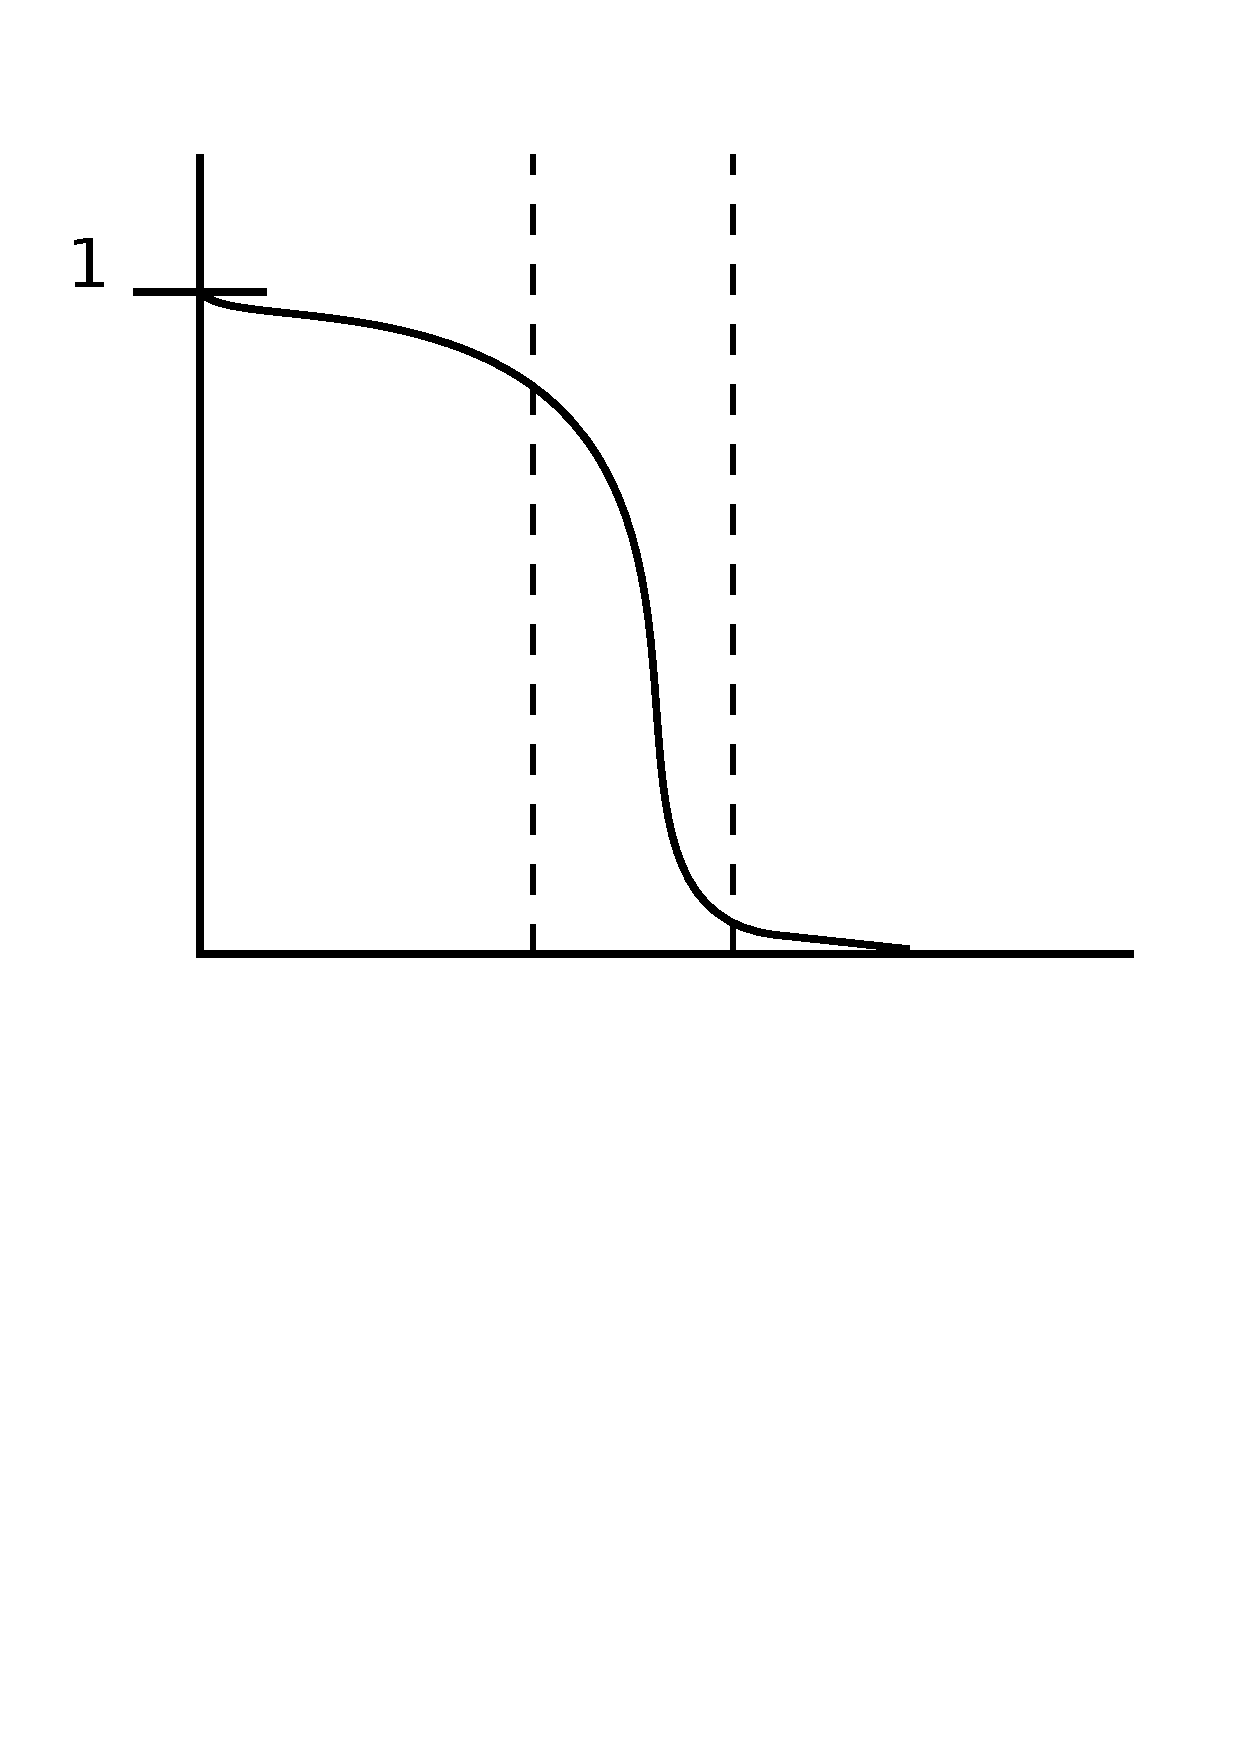
\includegraphics[width=0.3\textwidth]{Images/heuristik.pdf}
	\caption{Wir erwarten Funktionen, die stark abfallen. Der Erwartung nach findet der Abfall dabei lediglich in einem kleinen Intervall der Länge $\varepsilon$ statt}
	\label{figure_heuristik}
\end{figure}
\begin{example}\label{ex:c2e7s1}
	Betrachte \cref{prb:c2e7s1} im Einheitsintervall $\Omega=(0,1)$ mit $f=1$, $b=1$. Die Lösung lautet dann
	\[
		u_\varepsilon(x)\coloneqq x-\frac{e^{\frac{x}{\varepsilon}}-1}{e^{\frac{1}{\varepsilon}}-1}
	\]
	für jedes $\varepsilon > 0$.\par
	Wir beobachten, dass $u_\varepsilon$ steile Gradienten in der NÄhe von $x=1$ besitzt (eine so genannte \emph{Randschicht}).
	\begin{figure}[ht]
	\centering
		\includegraphics[width=0.3\textwidth]{Images/ergebnis.pdf}
		\caption{Die exakte Lösung. Im Intervall $[0,1-\varepsilon]$ verhält sich die Funktion wie $x\mapsto x$, in $[1-\varepsilon,1]$ wird der Linearteil der Lösung dann dominiert und es kommt zum steilen Abfall der Funktion}
		\label{figure_loesung}
	\end{figure}
	Daraus folgt, dass die Stabilitätskonstante des Problems mindestens wie $\frac{1}{\sqrt{\varepsilon}}$ wächst. Die Stabilitätskonstante ist dabei die Konstante auf der rechten Seite von \cref{eqn:c2e7s2}.
\end{example}
Wir betrachten die Galerkin-FEM erster Ordnung (P1-FEM) für \cref{prb:c2e7s1}. Sei $\mathcal{T}_h$ eine reguläre Triangulierung von $\Omega$ (polyhedral berandet). Wir suchen $u_{\varepsilon,h}\in P^1,0_0(\mathcal{T}_h)$, so dass 
\begin{equation}\label{eqn:c2e7s3}
	\forall v_h\in P^{1,0}_0(\mathcal{T}_h):\quad a_\varepsilon(u_{\varepsilon,h},v_h) = F(v_h).
\end{equation}
Unter den bereits gemachten Annahmen ist (\ref{eqn:c2e7s3}) wohlgestellt, siehe \cref{thm:c2e4s1}.\par
Falls $\Omega$ konvex ist, dann gilt $u_\varepsilon\in H^2(\Omega)\cap H^1_0(\Omega)$ und \cref{cor:c2e6s3} zeigt
\[
	\|u_\varepsilon-u_{varepsilon,h}\|_{H^1(\Omega)} \leq C_\varepsilon h\|f\|_{L^2(\Omega)}
\]
mit einer Konstante $C_\varepsilon$, die kritisch von $\varepsilon$ abhängt (d.h. die Konstante wächst wenn $\varepsilon$ gegen 0 geht). Es kann gezeigt werden, dass $C_\varepsilon \equiv \varepsilon^{-3}$. Damit müsste für $\varepsilon = 10^{-6}$ die Gitterweite bspw. als $h = 10^{-18}$ gewählt werden. Diese Abschätzung ist möglicherweise pessimistisch, jedoch zeigen viele Anwendungen, dass die bisher verwendete FEM nicht anwendbar ist:
\begin{example}\label{ex:c2e7s2}
	betrachte das 1d-Problem aus \cref{ex:c2e7s1} und FEM auf uniformem Gitter $\mathcal{T}_h$, $h=2^{-\ell}$, $\ell\in\N$. Wähle $\varepsilon = 2^{-8}$. Dann beobachten wir unphysikalische Oszillation in der numerischen Approximation $u_{\varepsilon,h}$, falls $h > \varepsilon$ ($\ell < 8$).
	\begin{figure}[ht]
	\centering
		\includegraphics[width=0.3\textwidth]{Images/oszillation.pdf}
		\caption{Das Ergebnis einer Standard-FEM: Die Lösungsfunktion (rot) oszilliert stark, dort wo sie es eigentlich nicht sollte}
		\label{figure_oszillation}
	\end{figure}
\end{example}
 Gibt es für $h>>\varepsilon$ eine ``vernünftige'' Methode?\\
 Idee zur Verbesserung dern umerischen Approximation in 1d:\par
 Ersetze die Bilinearform $a_\varepsilon$ in (\ref{eqn:c2e7s3})) durch $a_{\varepsilon+\delta}$ für einen \emph{Stabilisierungsparameter} $\delta \geq 0$. Wir addieren also künstliche Diffusion. 
 \begin{example}\label{ex:c2e7s3}
 	Betrachte wieder das Problem aus \cref{ex:c2e7s1} bzw \cref{ex:c2e7s2}. Sei $u_{\varepsilon,h,\delta}\in P^{1,0}_0(\mathcal{T}_k)$ die (FEM-) Lösung von
 	\[
 		\forall v_h\in P^{1,0}_0(\mathcal{T}_h):\quad \underbrace{a_{\varepsilon+\delta}(u_{\varepsilon,h,\delta}, v_h)}_{(\varepsilon+\delta)\int_\Omega\nabla u_{\varepsilon,h,\delta} \cdot\nabla v_h\dx + \int_\Omega b\nabla u_{\varepsilon,h,\delta}v_h\dx} = F(v_h)
 	\] 
 	Bei korrekter Wahl von $\delta$ ergibt eine FEM-Lösung, die nah an $u$ liegt.
 	\begin{figure}[ht]
 	\centering
 		\includegraphics[width=0.3\textwidth]{Images/stabilisiert.pdf}
 		\caption{Die Lösung des stabilisierten Problems ähnelt der analytischen Lösung, fällt jedoch früher ab. Offensichtlich ist die Wahl des Relaxationsparameters $\delta$ essentiell}
 		\label{figure_stabilisiert}
 	\end{figure}
 \end{example}
\end{document}